% ============================================================
% fig - ancilla layouts.tex
% Terminal postselection, one-ancilla and two-ancilla (conventional-site)
% check layouts on the conventional surface-code grid. The drawing is a
% standalone TikZ figure (paper-rework/layout-figure/ancilla-layouts.tex),
% compiled to figures/ancilla-layouts.pdf; the caption body lives here.
% Caption shortened by track hw (2026-11-13): the line styles are explained by
% the legend inside the figure, and the relay walk-through is in Appendix B.
% ============================================================
\begin{figure}[!tb]
  \centering
  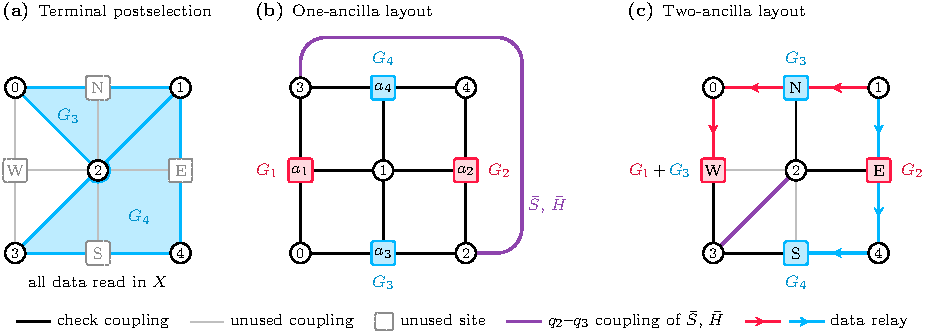
\includegraphics{figures/ancilla-layouts.pdf}% drawn at final size
  \caption{Stabilizer measurements of the $[[5,1,2]]_3$ code on the conventional surface-code grid of data qutrits (circles, labeled by their index) and ancilla sites (squares). Red marks the $Z$-type stabilizers $G_1$, $G_2$ and blue the $X$-type $G_3$, $G_4$. The label beside a site is what the site reads out once per check round, modulo three and up to a sign.
(a)~Terminal postselection uses no ancillas: the final $X$-basis readout of all data qutrits gives $G_3$ and $G_4$ (shaded).
(b)~One-ancilla layout, with $q_1$ at the center. Ancilla $a_j$ neighbors the three data qutrits of $G_j$, and the two-qutrit gates of $\bar H$ and $\bar S$ need a long-range coupling between $q_2$ and $q_3$.
(c)~Two-ancilla layout, with $q_2$ at the center and the sites N, W, E and S. $q_2$ and $q_3$ are diagonal neighbors, and $G_1$ and $G_4$ use two sites each. Arrows trace the data relay: N lends its part of $G_1$ to $q_0$, where W collects it, so that W reads $G_1$ shifted by the value of $G_3$ that N holds, and E lends its part of $G_4$ to $q_4$, where S collects it.}
  \label{fig:ancilla_layouts}
\end{figure}
